\documentclass[a0paper,12pt]{article}
\usepackage[landscape,top=5cm,bottom=3cm,right=5cm,left=5cm]{geometry}
\usepackage{graphicx}
\usepackage{standalone}
\usepackage{amsmath}
\usepackage[T1]{fontenc}
\usepackage{lmodern}
\usepackage{tikz}
\usepackage{tikzscale}
\usepackage{enumitem}
\usetikzlibrary{shapes,arrows}
\usetikzlibrary{arrows.spaced}
\usetikzlibrary{decorations.text}
\usetikzlibrary{spy,calc}
\usetikzlibrary{shapes.arrows}

\usepackage{color}
\usepackage{moresize}
\usepackage{lipsum} % dummy text
\usepackage{multicol}

\pgfdeclarelayer{background}
\pgfdeclarelayer{layer1}
\pgfdeclarelayer{layer2}
\pgfdeclarelayer{layer3}
\pgfdeclarelayer{foreground}

\newenvironment{Figure}
  {\par\medskip\noindent\minipage{\linewidth}}
  {\endminipage\par\medskip}

% This macro creates header.
\newcommand{\HEADING}[1]
{
    %\includegraphics[scale=0.35]{./images/heading.png}
    %\MOOSELOGO
    \fontsize{2.2cm}{1cm}\selectfont \textcolor{black}{#1}
    \vspace{0.5cm}
}

\newcommand{\SECTION}[1]
{
    {\fontsize{1.75cm}{1.5cm}\selectfont \textsc{\textcolor{blue}{#1}}\par}
}

\newcommand{\CAPTION}[1]
{
    {\fontsize{1cm}{1cm}\fontfamily{\sfdefault}\selectfont {\textcolor{black}{#1}}\par}
}

\newcommand{\TEXT}[1]
{
   { \fontsize{1.4cm}{1.0cm}\fontfamily{\sfdefault}\selectfont {#1}\par }
}

\newcommand{\ITEM}[1]
{
    {\fontsize{1.2cm}{1.2cm}\fontfamily{\sfdefault}\selectfont {#1}\par }
}

\newcommand{\MOOSE}[0]{\textsc{\textcolor{black}{MOOSE}}}

\newcommand{\MOOSELOGO}[0]{
    \tikz \node[inner sep=1mm] {\includegraphics[scale=0.6]{./images/moose_logo_tiny.png}}; 
}

\tikzset{
  every overlay node/.style={
    draw=black,fill=white,rounded corners,anchor=north west,
  },
}
% Usage:
% \tikzoverlay at (-1cm,-5cm) {content};
% or
% \tikzoverlay[text width=5cm] at (-1cm,-5cm) {content};
\def\tikzoverlay{%
   \tikz[baseline,overlay]\node[draw=white,every overlay node]
}%

\begin{document}

\begin{tikzpicture}[remember picture,overlay] 
    \node[opacity=1.0] (background) at (current page.center) {
        
\includegraphics[width=\paperwidth,height=\paperheight]{./background/background.jpg}
    };
\end{tikzpicture}

\begin{tikzpicture}
    \centering
    \node[] (logo) { 
        
\includegraphics[height=6cm]{./images/NCBS-Logo.jpg}
    };

    \node [] (title) at ([xshift=40cm]logo.east) {
        \fontsize{4cm}{1em}\selectfont \textcolor{black}{Modelling Memory Across
            Scales}
    };

    \node[] (authors) at ([yshift=-1cm]title.south) {
        \fontsize{1.5cm}{1em}\selectfont Subhasis Ray, Harsha Rani, Sahil Moza,
        Aditya Gilra,  Aviral Goel, Dilawar Singh, Upinder Bhalla
    };

    \node [] (mooselogo) at ([xshift=20cm]title.east) {
        \includegraphics[height=6cm]{./images/moose_logo_tiny.png}
    };
\end{tikzpicture}

%% Three columns
\vspace{5cm}
\setlength{\columnsep}{5.5cm}
\begin{multicols}{3}
    
%%%%%%%%%%%% Column 1
\begin{Figure}
    \HEADING{1. Why Multiscale?}

    \begin{Figure}
        %\begin{tikzpicture}[]
    \LARGE
    \def\lengthScaleFactor{1.6}
    \def\timeScaleFactor{1.6}

    \newcommand\scaleNode[1]{
        (0, #1*\timeScaleFactor)
    }

    \coordinate (sizeRoot) at (0, 1);
    \coordinate (sizeends) at (0,-1+11*\lengthScaleFactor);
    \coordinate (timeRoot) at (1,0);
    \coordinate (timeends) at (1+11*\timeScaleFactor, 0);


    \draw[-fast cap, blue!20!white, line width=6ex]  (timeRoot) to[] (timeends);
    \draw[-fast cap, blue!20!white, line width=6ex]  (sizeRoot) to[] (sizeends);


    \node[] (nm) at (0,1) {$10^{-9}m$};
    \node[] (um) at (0,5) {$10^{-6}m$};
    \node[] (mm) at (0,9) {$10^{-3}m$};
    \node[] (m) at (0,13) {$10^{-0}m$};

    \node[] (us) at (1.5,0) {$\mu$ sec};
    \node[] (ms) at (4.5,0) {$m$ sec};
    \node[] (s) at (7.5,0) {sec};
    \node[] (hrs) at (10.5, 0) {hours};
    \node[] (days) at (13.5, 0) {days};

    %% Distance between images and y-axis.
    \def\shifty{-3.0cm}

    \node[] (n1) at ([xshift=\shifty,yshift=0cm]nm) {
        \includegraphics[width=0.1\textwidth]{images/8tim_TIM_barrel.png}
    };

    \node[] (n2) at ([xshift=\shifty,yshift=0cm]um) {
        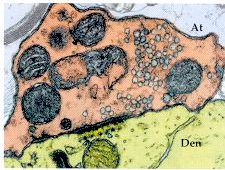
\includegraphics[width=0.1\textwidth]{images/dendrite.png}
    };

    \node[] (n3) at ([xshift=\shifty,yshift=-1cm]mm) {
        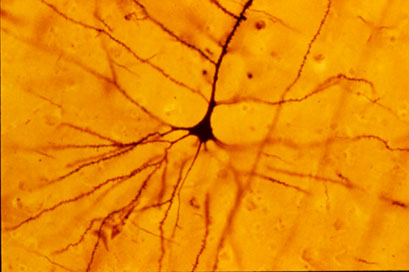
\includegraphics[width=0.1\textwidth]{images/GolgiStainedPyramidalCell.jpg}
    };

    \node[] (n4) at ([xshift=\shifty,yshift=1cm]mm) {
        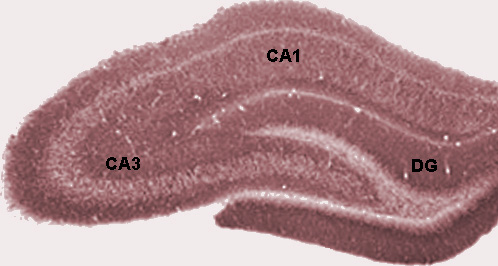
\includegraphics[width=0.1\textwidth]{images/HippocampalRegions.jpg}
    };

    \node[] (n5) at ([xshift=\shifty,yshift=-1.0cm]m) {
        \includegraphics[width=0.1\textwidth]{images/brain.png}
    };

    \node[opacity=0.5, rectangle, minimum width=12cm, minimum height=7.0cm,
    fill=blue!20, rounded corners] (chemical) at (9.0,4.5) {};

    \node[] (caption) at ([yshift=-1cm]chemical.north) {\LARGE Chemical};

    \node[opacity=0.5, rectangle, minimum width=4cm, minimum height=7cm, fill=red!20, rounded corners] 
    (electrical) at (4.0, 11.0) {};

    \node[] at (electrical.center) {\LARGE Electrical};


    % Put chemical network here
    \node[] (network) at (7.0,4.0) {
        \includegraphics[width=5cm]{images/chemical_reactions.png}
    };

    \node[] (chromosome) at (11.0,6.0) {
        
\includegraphics[width=5cm]{images/chromosome.png}
    };

    \node[fill=red!1] (text) at ([xshift=5cm]electrical.east) {
        \begin{minipage}{0.3\textwidth}
            \large
            \begin{itemize}
                \item $10^{11}$ cells, $10^{15}$ synapses, $10000$? reactions per synapse
                \item Electrical events: $< 1$ ms,  Chemical events: $1\;
                    \text{sec} \rightarrow 1000\; \text{sec}$
            \item Structural events: $100\; \text{sec} \rightarrow \text{months}$
        \item Lifetime of a protein: days, a neuron: 100 years, a memory: 100 years
    \end{itemize}
\end{minipage}
        };
    \end{tikzpicture} %



        \begin{itemize}
            \item \TEXT{Memory and plasticity involve brain mechanisms from molecular scale
                    to enormous networks.}

            \item \TEXT{We have developed \textcolor{black}{\textsc{MOOSE}}
                    the Multiscale Object Oriented Simulation
                    Environment, to model plasticity across scales.}

        \end{itemize}

     \begin{tikzpicture}[
        spy using outlines={circle
            , magnification=10, connect spies
        }
                 ]
         \centering
         \node [] (image) at (0,-1) {
             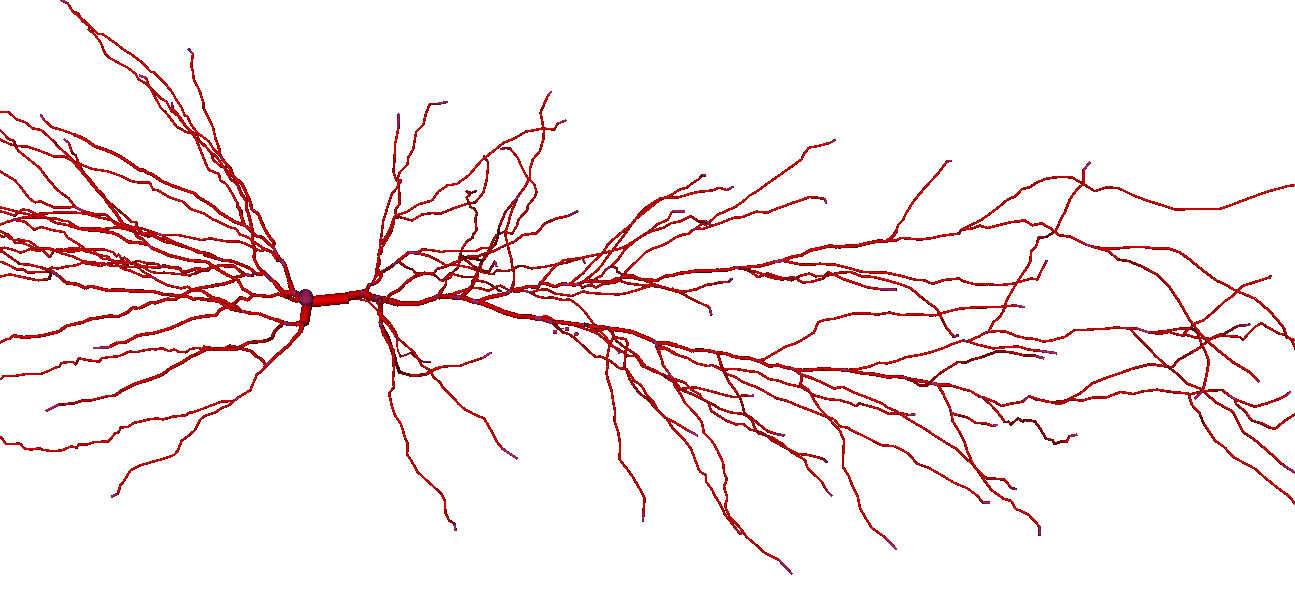
\includegraphics[scale=0.2,angle=-30]{./images/ca1_neuron.png}
         };

         \foreach \i in {-3,...,3}
         \foreach \j in {-3,...,3}
         {
             \node[fill=blue!40,opacity=0.3,thin,inner sep=0pt, minimum size=3mm,circle] (n\i\j) at (\i, \j) {};
         };

         \spy[blue, size=3cm] on (1.65, -1.5) in node[left] at (7,3);
         \node[below=4cm,text width=0.3\textwidth] {\CAPTION{A single neuron is
                 embedded in lattice of neural network}};

         %% Cool. Now create a 3d compartment model here.
         \begin{scope}[xshift=11cm, yshift=3cm
             , compartment/.style={cylinder
                 , draw
                 , cylinder uses custom fill
                 , cylinder end fill = red!35
                 , cylinder body fill = red!40
                 , inner sep = 3mm
                 , minimum height = 1cm
                 , minimum width = 1cm 
             }
             , spine/.style={cylinder 
                 , fill = blue!20
                 , inner sep=1mm
                 , minimum height=1mm
                 , minimum width=3mm
             }
             , branch/.style={cylinder
                 , draw
                 , cylinder uses custom fill
                 , cylinder end fill = red!35
                 , cylinder body fill = red!40
                 , minimum height = 1.5cm
                 , minimum width = 0.5cm
                 , inner sep = 1mm
             }
             ]

             \node[compartment] (c1) {};
             \node[compartment] (c2) at (c1.east) {};
             \node[compartment] (c3) at (c2.east) {};

             \node[branch,rotate=45] (b1) at ([xshift=4mm,yshift=2mm]c3.before top) {};
             \node[branch,rotate=-45] (b2) at ([xshift=1mm, yshift=-7mm]c3.base east) {};

             % Spines
             \node[spine, inner sep=1mm, rotate=135] (s11) at (b1.north east) {};
             \node[spine, inner sep=1mm, rotate=135] (s12) at ([xshift=3mm]b1.south east) {};

             \node[spine, inner sep=1mm, rotate=45] (s21) at (b2.north east) {};
             \node[spine, inner sep=1mm, rotate=45] (s22) at ([xshift=-3mm]b2.south east) {};

         \end{scope}

         %% Scope to draw chemisty 
         \begin{scope}

             \node[] (chemical) at ([yshift=-5.5cm]c2.south) {
                 \includegraphics[width=0.35\textwidth, trim=5mm 5mm 5mm 5mm, clip]{./images/chemical_reactions.png}
             };

             %%  
             \node [above] (chemicallabel) at ([yshift=-2cm]c1.south) {\LARGE{
                     Chemical models}};

             \draw[o-o] (c1.center) to [bend right] (chemicallabel.center);
            
             %% Add transportation model.
             \node[] (transport) at ([xshift=7cm,yshift=-3cm]s12.north) {
                 \includegraphics[width=0.3\textwidth]{./images/transport_mechanism.png}
             };

             \node[] (tlabel) at ([xshift=0.5cm, yshift=-1cm]transport.north) {\LARGE{Trafficking
                     models}};

             \draw[o-o] (s21.center) to [bend left] (tlabel) ;

         \end{scope}


     \end{tikzpicture} 
    \end{Figure}


    \HEADING{2. Multiscale Modeling in MOOSE}
    \edef\figwidth{0.12\textwidth}
    \vspace{-1cm}
   
    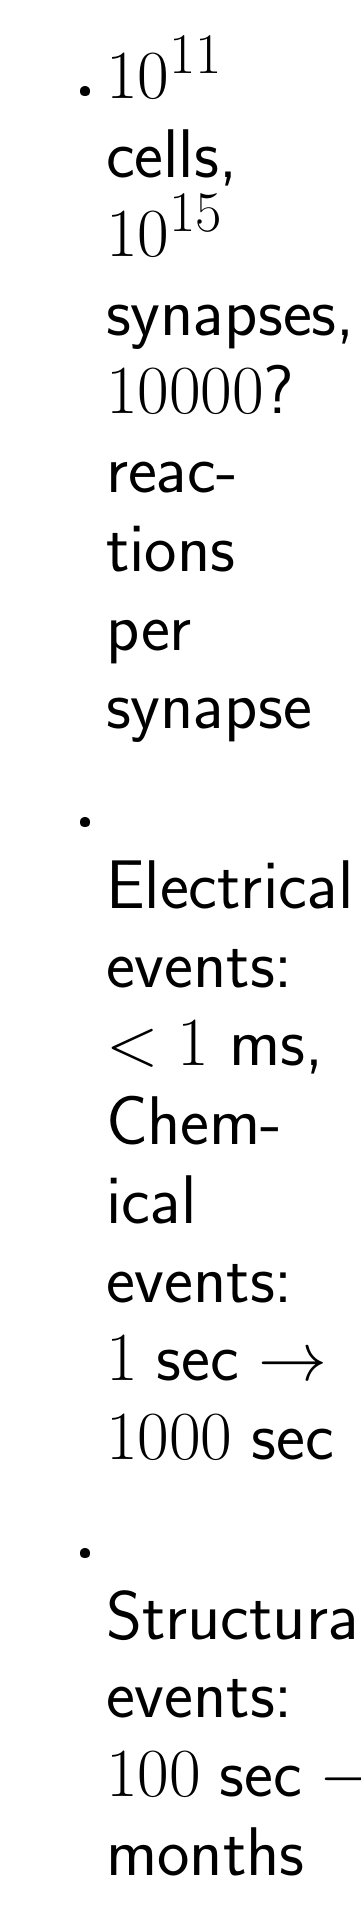
\begin{tikzpicture}
        \node[] (text) {
            \begin{minipage}{0.3\textwidth}
                \begin{itemize}
                    \item \CAPTION{$10^{11}$ cells, $10^{15}$ synapses, $10000$?
                            reactions per synapse}
                    \item \CAPTION{Electrical events: $< 1$ ms,  Chemical events: $1\;
                        \text{sec} \rightarrow 1000\; \text{sec}$}
                    \item \CAPTION{Structural events: $100\; \text{sec}
                        \rightarrow \text{months}$}
                \end{itemize}
            \end{minipage}
        };
    \end{tikzpicture} %
    \begin{tikzpicture}[
        image/.style = {xslant=0.0,yslant=0.0}
        ]
        \LARGE
        \def\lengthScaleFactor{1.4}
        \def\timeScaleFactor{1.2}

        \newcommand\scaleNode[1]{
            (0, #1*\timeScaleFactor)
        }

        \coordinate (sizeRoot) at (0, 1);
        \coordinate (sizeends) at (0,-1+10*\lengthScaleFactor);
        \coordinate (timeRoot) at (1,0);
        \coordinate (timeends) at (1+11*\timeScaleFactor, 0);


        \draw[-fast cap, yellow!50, line width=4ex]  (timeRoot) to[] (timeends);
        \draw[-fast cap, yellow!50, line width=4ex]  (sizeRoot) to[] (sizeends);


        \node[] (nm) at (0,1) {$nm$};
        \node[] (um) at (0,3.5) {$\mu m$};
        \node[] (mm) at (0,7) {$mm$};
        \node[] (m) at (0,10.5) {$m$};

        \node[] (us) at (1.5,0) {$\mu$ sec};
        \node[] (ms) at (4.0,0) {$m$ sec};
        \node[] (s) at (6.5,0) {sec};
        \node[] (hrs) at (8.5, 0) {hours};
        \node[] (days) at (11.5, 0) {days};

        %% Distance between images and y-axis.
        \def\shifty{-3.0cm}

        \node[image] (n1) at ([xshift=\shifty,yshift=0cm]nm) {
            \includegraphics[width=0.1\textwidth]{images/8tim_TIM_barrel.png}
        };

        \node[image] (n2) at ([xshift=\shifty,yshift=0cm]um) {
            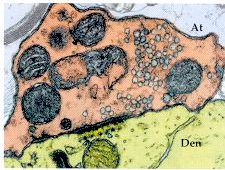
\includegraphics[width=0.1\textwidth]{images/dendrite.png}
        };

        \node[image] (n3) at ([xshift=\shifty,yshift=-1cm]mm) {
            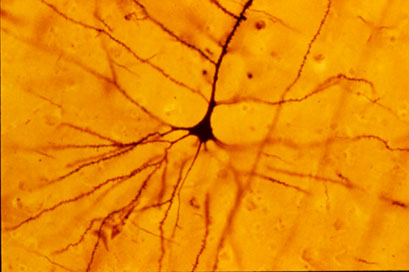
\includegraphics[width=0.1\textwidth]{images/GolgiStainedPyramidalCell.jpg}
        };

        \node[image] (n5) at ([xshift=\shifty,yshift=-1.0cm]m) {
            \includegraphics[width=0.1\textwidth]{images/brain.png}
        };

        \node[image] (n4) at ([xshift=\shifty,yshift=1cm]mm) {
            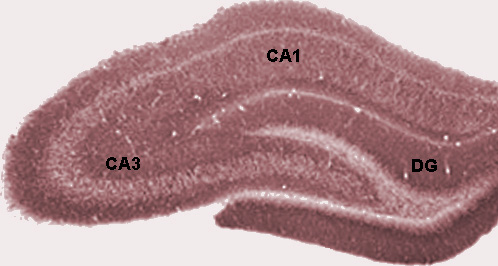
\includegraphics[width=0.1\textwidth]{images/HippocampalRegions.jpg}
        };


        \node[rectangle, minimum width=12cm, minimum height=6.0cm,
            draw, rounded corners] (chemical) at (9.0,4.5) {};

        \node[] (caption) at ([yshift=-1cm]chemical.north) {\LARGE Chemical};

        \node[rectangle, minimum width=3cm, minimum height=4.5cm
            , draw, rounded corners
            ] (electrical) at (3.5, 9.0) {};

        \node[] at (electrical.center) {\LARGE Electrical};


        % Put chemical network here
        \node[] (network) at (7.0,4.0) {
            \includegraphics[width=5cm]{images/chemical_reactions.png}
        };

        \node[] (chromosome) at (12.0,5) {
            
\includegraphics[width=5cm]{images/chromosome.png}
        };
    \end{tikzpicture} 

    %% Modular solvers available in MOOSE
    \def\figwidth{0.15\textwidth}
    \def\captionwidth{0.2\textwidth}
    \begin{tikzpicture}
        \node[] (stochastic) {
            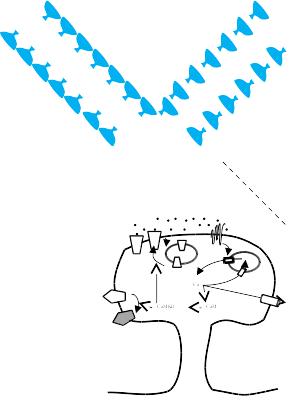
\includegraphics[width=\figwidth]{./images/stochastic_solver.png}
        }; 
        \node[text width=\captionwidth] at ([yshift=-1cm]stochastic.south)
            {\CAPTION{Reaction at single molecule level}
            };
        \end{tikzpicture} \hfill %
        \begin{tikzpicture}
            \node[] (ksolve) { %at ([xshift=4cm]stochastic.east) {
                \includegraphics[width=\figwidth]{./images/ksolve_dsolve.png}
            };
            \node[text width=\captionwidth] at ([yshift=-1cm]ksolve.south) {\CAPTION{Reaction Diffusion Solver}};
        \end{tikzpicture} \hfill %
        \begin{tikzpicture}
            \node[] (hsolve) { % at ([xshift=4cm]ksolve.east) {
                \includegraphics[width=\figwidth]{./images/hsolve.png}
            };
            \node[text width=\captionwidth] at ([yshift=-1cm]hsolve.south) {\CAPTION{Electrical: Hines Solver}};
        \end{tikzpicture}

        \edef\figwidth{0.27\textwidth}
        \begin{tikzpicture}
            \node[] (signalling)  {
                \includegraphics[width=\figwidth]{./images/poster_editView.png}
            };
            \node [text width=\captionwidth, below=2.7cm] (captionC)  {\CAPTION{Signalling Model}};
        \end{tikzpicture}%
        \begin{tikzpicture}
            \node [] (moose_cell) {
                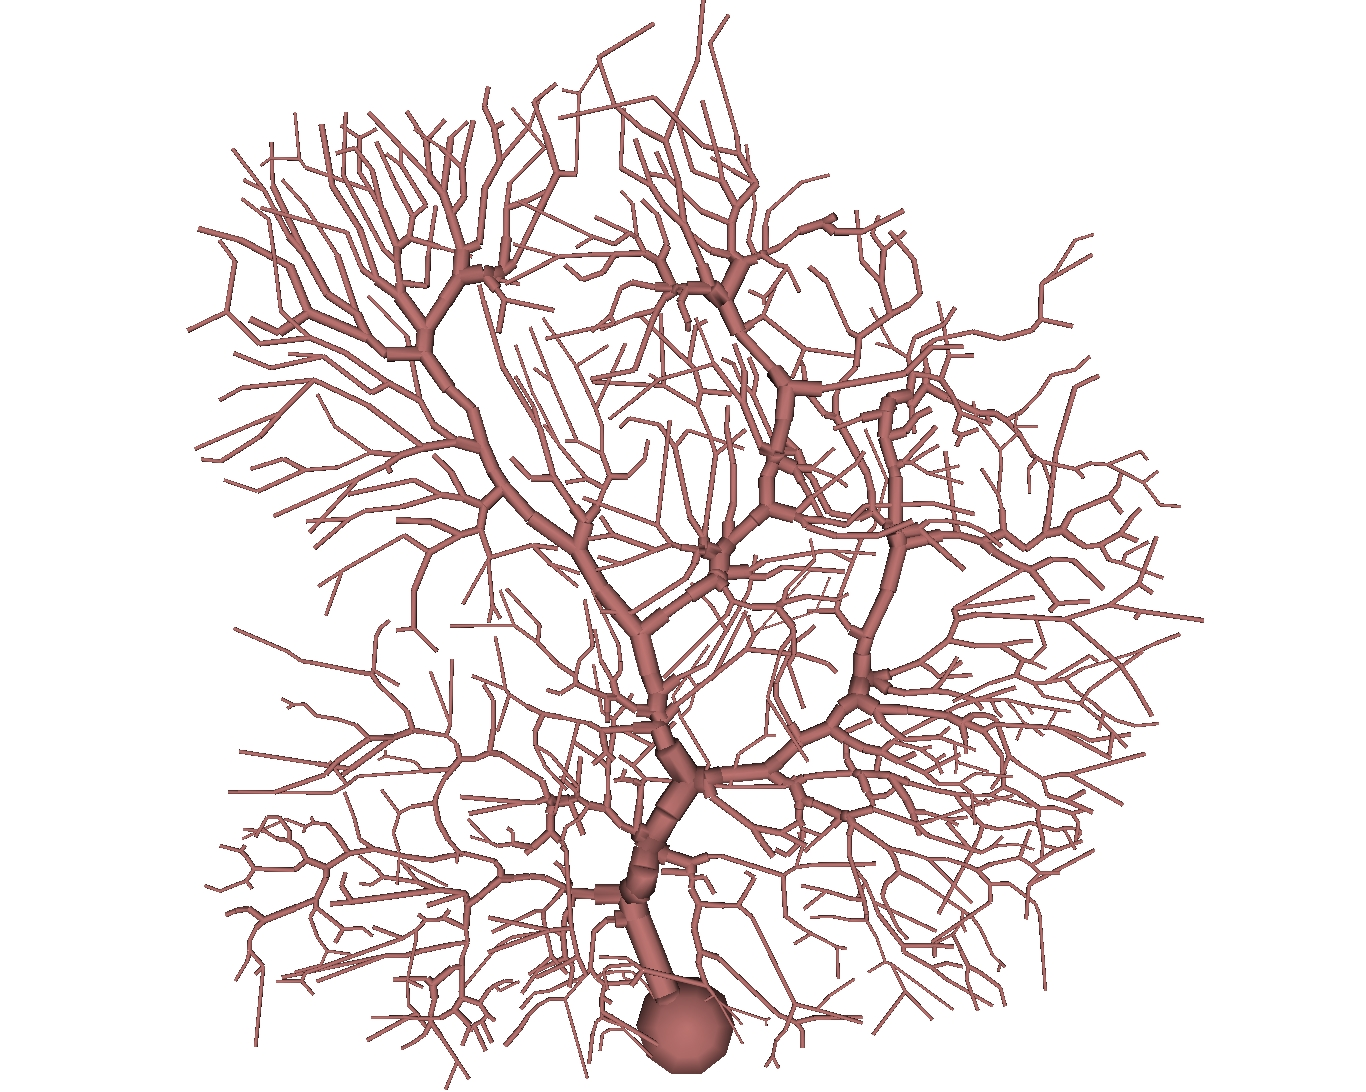
\includegraphics[width=\figwidth]{./images/_1_7.jpeg}
            };
            \node [text width=\captionwidth,below=3.5cm] (captionA) {\CAPTION{Single Neuron Model}};
        \end{tikzpicture}%
    \begin{tikzpicture}
        \node[] (olfaction) {
            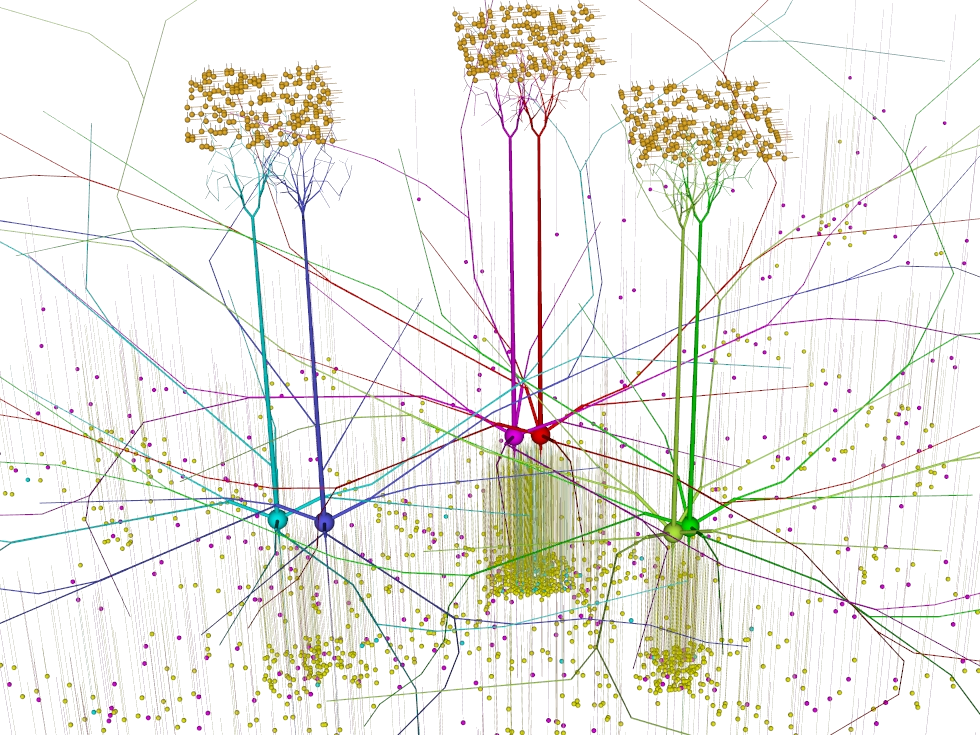
\includegraphics[width=\figwidth]{./images/fullmodel_moogli.png}
        };
        \node [text width=\figwidth, below=2.7cm] (captionB) {\CAPTION{Olfactory
                bulb model}};
    \end{tikzpicture}

\end{Figure}

\columnbreak
\HEADING{3. Some projects using MOOSE}
\begin{Figure}
    \edef\figwidth{0.95\textwidth}
    \SECTION{3.1 Olfactory bulb project}
    \TEXT{ Network coding and computation in olfaction and somatosensory
        cortex. It explains linear coding and phase-decorrelation and
        predicts connectivity, lateral dendrite output structure.}

    \begin{tikzpicture}
        \node[] (aditya) {
            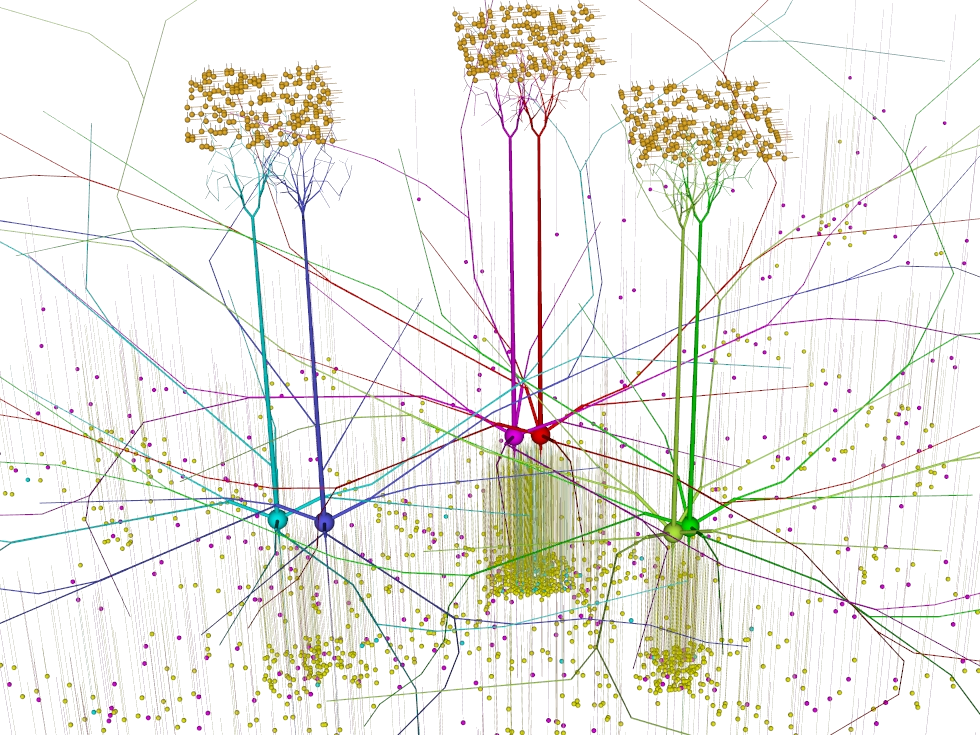
\includegraphics[width=\figwidth]{./images/fullmodel_moogli.png}
        };
    \end{tikzpicture}

    \begin{tikzpicture}
        \node[] (result) {
            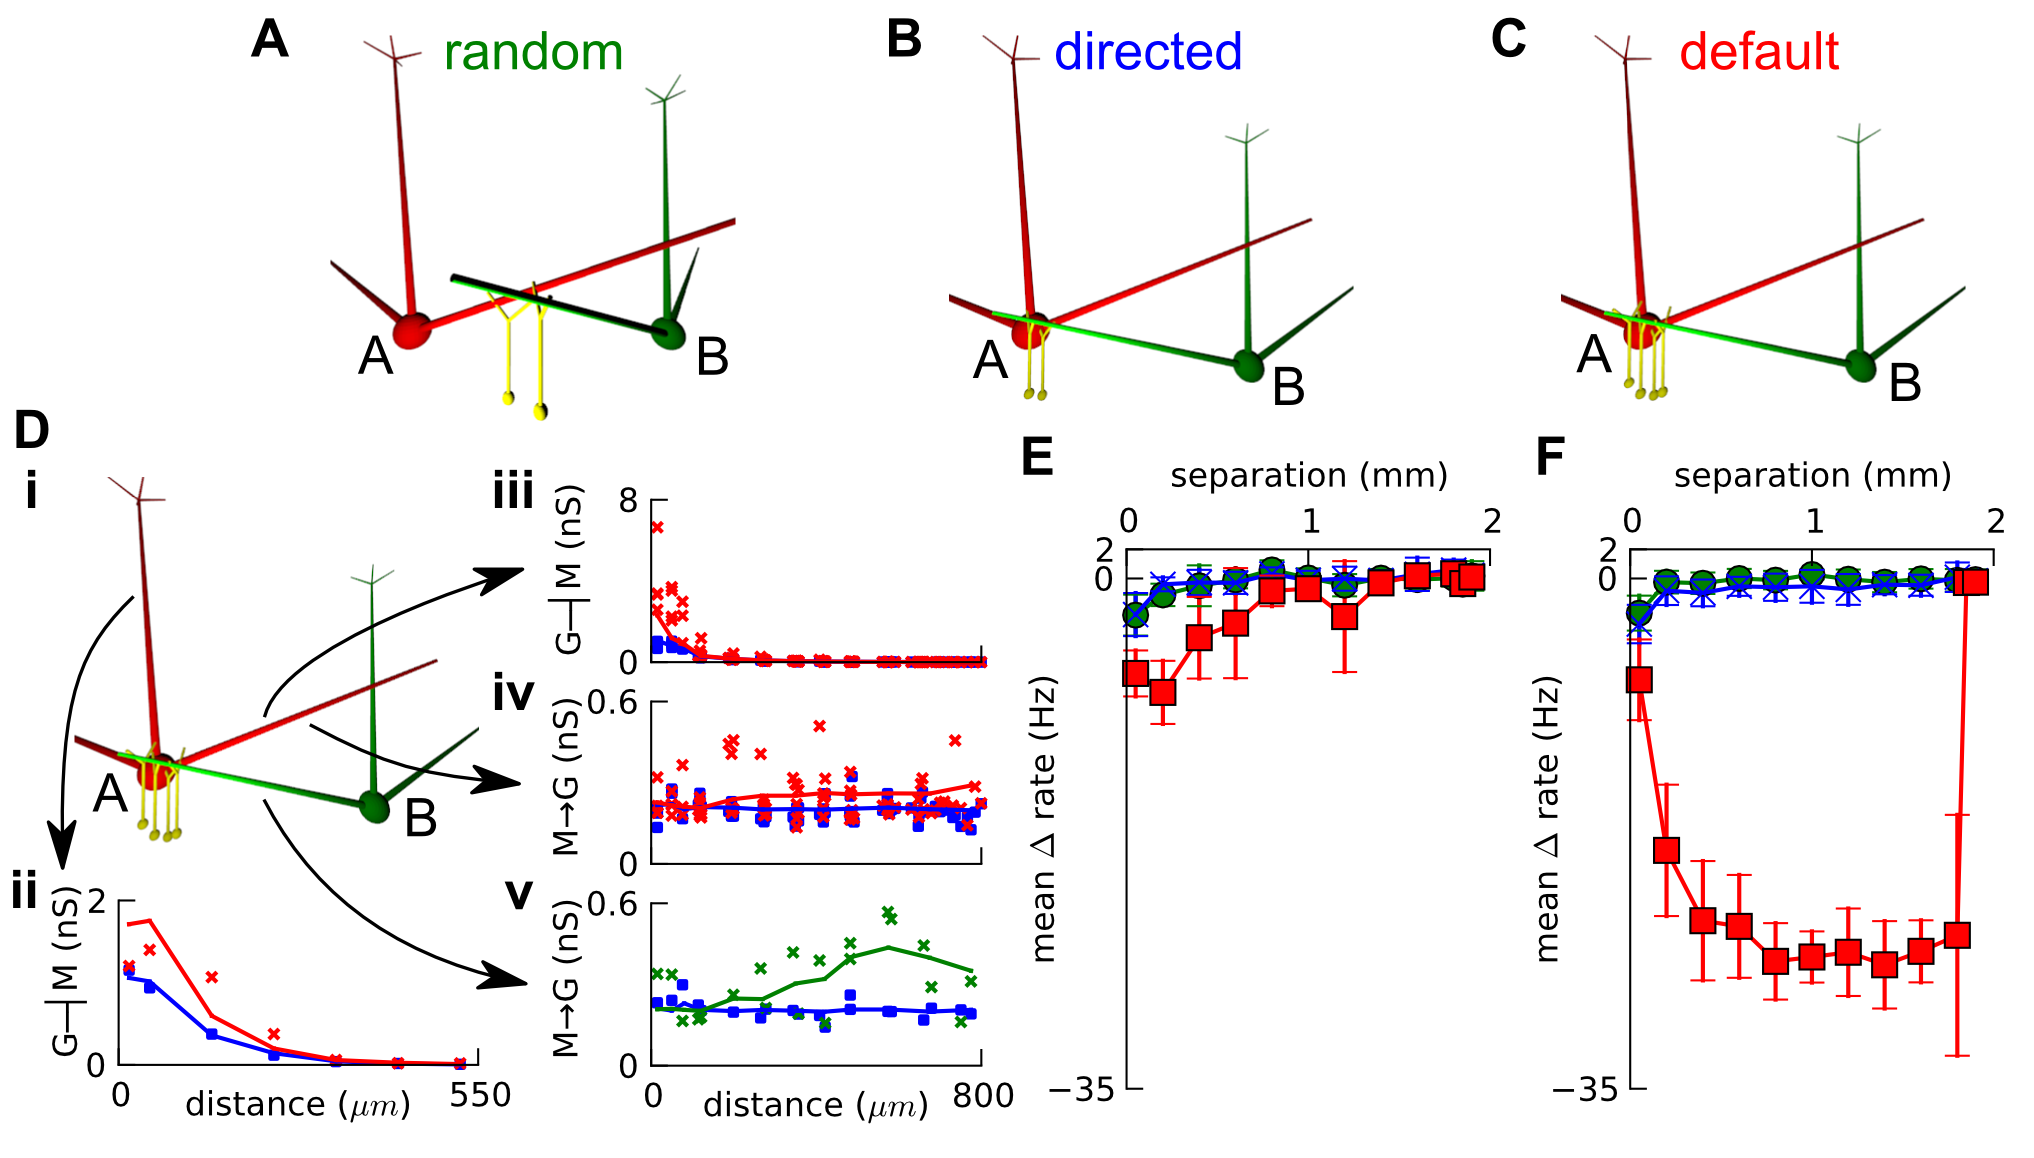
\includegraphics[width=\figwidth,trim=0cm 0cm 0cm 3.5cm,clip]{./images/aditya_work.png}
        };
    \end{tikzpicture}

    %% One more model here.
    \SECTION{3.2 Signalling Pathways}
    \begin{tikzpicture}
        \node[] (robust) {
            \includegraphics[width=0.6\textwidth]{./images/chemical_model.png}
        };
    \end{tikzpicture}%
    \begin{tikzpicture}
        \node [] (chemical_result) {
            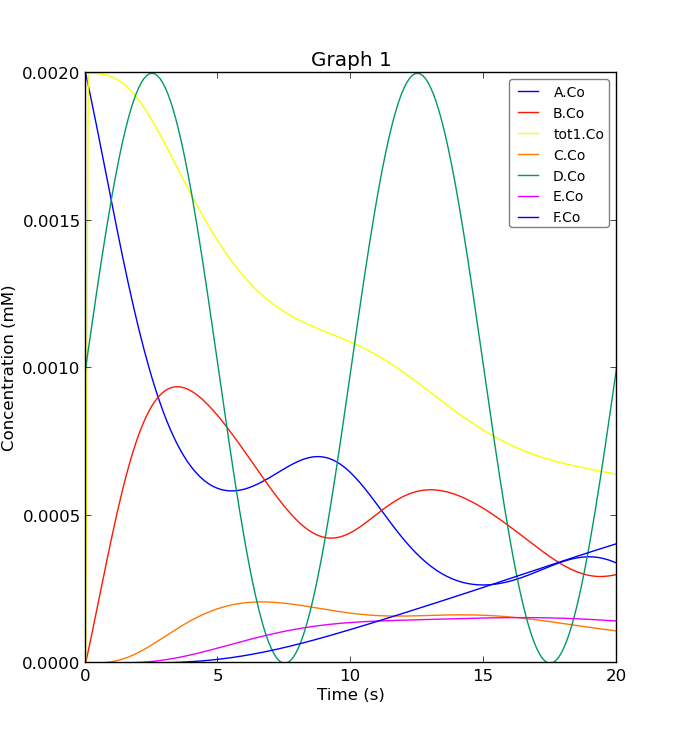
\includegraphics[width=0.32\textwidth]{./images/chemical_result.png}
        };
    \end{tikzpicture}

    %\SECTION{3.3 Single column Thalamacortical Model}

    %\begin{tikzpicture}
        %\node [fill=yellow!20] (subha) {
            %\includegraphics[width=0.12\textwidth]{./images/thalamocortical.png}
        %};
    %\end{tikzpicture}%
    %\begin{tikzpicture}

        %%\node [] (subha2) at (subha.east) {
            %%\includegraphics[width=0.2\textwidth]{./images/celltypenetwork.pdf}
        %%};

        %\node[] (subha3) at ([xshift=5cm]subha.east) {
            %\includegraphics[width=0.25\textwidth]{./images/thalamocorticalcircuit.png}
        %};
    %\end{tikzpicture}


\end{Figure}

%% Column 3
\begin{Figure}
    
    \SECTION{3.3 Robustness of Chemical Switches}

   \begin{tikzpicture}
        \node [] (model) {
            \includegraphics[width=0.3\textwidth]{./images/model.png}
        };
    \end{tikzpicture} %
    \begin{tikzpicture}
        \node [] (timeline) {
            \includegraphics[width=0.6\textwidth]{./images/timeline.png}
        };
    \end{tikzpicture}

    \begin{tikzpicture}
        \node [] (timeseries) {
            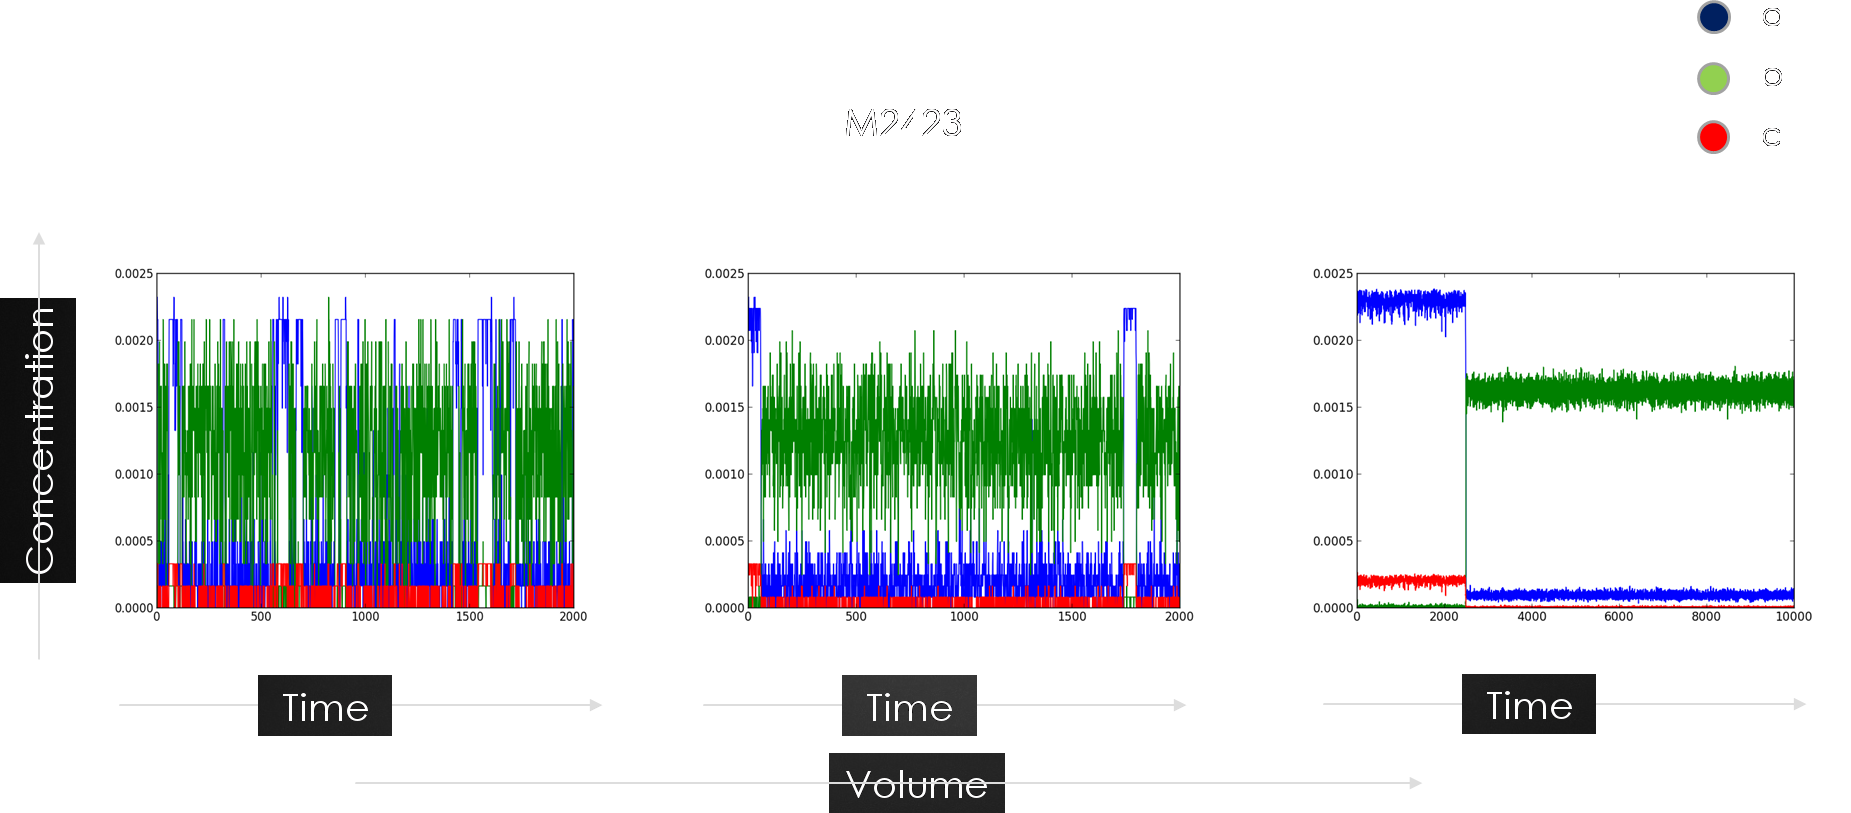
\includegraphics[trim=0 0 0 3cm,width=\textwidth,clip]{./images/TimeSeries.png}
        };
        \node [] (caption) at ([xshift=-4cm,yshift=0cm]timeseries.north) {
            \CAPTION{Stochastic simulation of bistable chemical models}
        };

        \node[inner sep=1mm, minimum size=1.5cm,fill=blue,circle] (a) at
        (caption.east) {\Huge \textcolor{white}{a}};
        \node[inner sep=1mm, minimum size=1.5cm,fill=green,circle] (b) at
            ([xshift=2cm]a.east)  {\Huge b};
        \node[inner sep=1mm, minimum size=1.5cm,fill=red,circle] (c) at
        ([xshift=2cm]b.east) {\Huge c};

    \end{tikzpicture}

    
    \begin{tikzpicture}
        \node[] (ktseries) {
            \includegraphics[width=0.8\textwidth]{./images/KT_statistic_crop.png}
        };

    \end{tikzpicture}


    \HEADING{4. Summary}

    \TEXT{\bf We use models to,}
    \begin{itemize}
        \item \TEXT{Integrate many scales of neuronal data with basic
            physical/chemical principles.}
        \item \TEXT{Explain phenomena of plasticity, activity and neuronal
                coding.}
        \item \TEXT{Predict circuit mechanisms, plasticity rules, and emergent
            phenomena such as \emph{decorrelation}, \emph{robustness}, and
            \emph{memory decay}.}

    \end{itemize}

\end{Figure}

\end{multicols}
\end{document}
